\documentclass[BSP,english,oneside]{gucthesis}

\usepackage[utf8]{inputenc}		%UTF-8 encoded inlude files
\usepackage[pdftex]{graphicx,hyperref}
\usepackage{color}

% Remove '%' in front of \renewcommand the parent command

% Create command for commenting
\newcommand{\comment}[1]{\textcolor{blue}{\emph{#1}}}
%\renewcommand{\comment}[1]{}

% Create command for todo things
\newcommand{\todo}[1]{{\color{green}#1}}

% Norwegian Characters,  needs the {} or to be separate from the next letters
% \o{}   \aa{}   \ae{}   so at the end of a word you can use \o  \aa   \ae
% \O{}   \AA{}   \AE{}   you can also just leave a space and latex will remove it
%                        eg,  H\o gskolen i Gj\o vik


\begin{document}

\thesistitle{AR Cubes}
\thesisauthor{Per Kristian Warvik}
\thesisauthorA{Daniel Granerud}
\thesisauthorB{Jakob Sand Svarstad}
%\thesisauthorC{}
\thesissupervisor{Simon McCallum}
%\thesissupervisorA{} %second supervisor

\gmtkeywords{Thesis, AR, cubes, IMT, cognitive, Augmented Reality}
\gmtdesc{Minigame environment with cubes in an augmented reality setting.}
\gmtnumber{-} % this is the number given to your project. May not be used  

\gmtoppdragsgiver{\GUC, Costas Bolentsis}
\gmtcontact{Costas Bolentsis, @hig.no, 12345678}




\thesisdate{\gucthesisdate}
\useyear{25.05.2014}

\gmtappnumber{} %numebr of appendixes
\gmtpagecount{} %currently auto calculated but might be wrong


\thesistitleNOR{AR Cubes}
\gmtkeywordsNOR{Norway, Norsk}
\gmtdescNOR{Denne oppgaven omhandler et milj\o{}  for \aa{} lage mini-spill som
kan brukes til kognitiv forskning. Teknologien som brukes er Augmented Reality.
Spillene l\o ses ved \aa{} flytte p\aa{} kuber med mark\o rer.}



\makefrontpages

\chapter*{Preface} %the * means do not give the chapter a number
\label{chap:preface}

We would like to thank Erik Hjelm\aa{}s for motivating the development of a \LaTeX{} template
 for GUC's master's theses.  This has expanded to include Bachelor and perhaps soon the PhD 
 template.
 
 



\tableofcontents
\listoffigures
\listoftables

% Put introduction here
\chapter{Introduction}
\label{chap:introduction}

Starting in 2005, \GUC (GUC) was given the
right to issue Master diplomas. As a consequence of this, directions
for the master's thesis have been developed~\cite{GUCMaster},
including guidelines for the typographical details. These detailed
typographical rules have been implemented in the
\texttt{gucmasterthesis} \LaTeX\ document class.

The purpose of this document is to provide an example and description
on how this class file can be used.

This was then extended to include bachelor project by Simon McCallum.
The package has changed names and version number it is now called
\texttt{gucthesis}
v\gucthesisversion\ as of \gucthesisdate.


\chapter{Packages}
\label{chap:packages}

The \texttt{gucthesis} is built upon the standard \LaTeX\
\texttt{report} class. All commands from the \texttt{report} class can
be used, with the two exceptions of \verb+\subsubsection+ and
\verb+\paragraph+. This is because there should only be three
levels of headings according to the guidelines~\cite{GUCMaster}.

\section{Packages Used by gucthesis}
\label{sec:packages}

In addition to the \texttt{report} document class,
\texttt{gucthesis} makes direct use of the following packages
that must hence be present:
\begin{description}
	\item[geometry:] used for setting the sizes of the margins and
  	headers.
	\item[fontenc:] used with option \texttt{T1} for forcing the Cork font
  	encoding (necessary for the Charter font).
	\item[charter:] load Charter as the default font.
	\item[euler:] load the Euler math fonts.
	\item[babel:] to load language specific strings. Reasonable options
	  include \texttt{british}, \texttt{american}, \texttt{norsk},
	  \texttt{nynorsk} and \texttt{samin}.
\end{description}

\section{Other Relevant Packages}
\label{sec:otherpackages}

The author of a thesis might want to use a bunch of different packages
to those described in Section~\ref{sec:packages} in order to have all features needed for their document. 
In particular, it is advised to use the following:
\begin{description}
	\item[inputenc:] to allow \LaTeX\ to use more than 7-bit ASCII for its
	  input. Most often, the option \texttt{latin1} will do.
	\item[graphicx:] to include graphics.
	\item[hyperref:] this is a very nice package that makes cross links in
	  pdf documents. Use with option \texttt{dvips} or \texttt{pdftex}
	  in accordance with the driver that you use. Unfortunately, hyperref
	  is not completely bugfree\dots
\end{description}

\chapter{Structural Elements}
\label{chap:structural}

The title of the thesis should be set using the \verb+\thesistitle+
command, and the date of the thesis should be set using the
\verb+\thesisdate+ command. This makes the title and date appear in
the running header, like in this document.

\section{Page Layout}

The geometry of the page has been set using the \verb+\geometry+
command.

\section{Fonts}

Due to limited \LaTeX\ support for the Georgia font, Charter has been
chosen instead. For mathematical formula, the Euler fonts are used,
since they blend more nicely with the Charter than the standard
\LaTeX\ fonts: 
$$
 f(x) = \int_0^x g(\tau)\,d\tau
$$

For inline math you can use $\backslash{}($ and $\backslash{})$ for example \( f(x)= \frac{x^2}{1+x^2} \).  
This also allows you to use $\slash$ and $\backslash$. You need to include the \{\} when you want the special
character to have other letters immediately after it.

\section{Sectioning Commands}

The standard \LaTeX\ sectioning commands are used for both numbered
and unnumbered sections. The top level is given by the \verb+\chapter+
command. This starts a new right page. The two lower levels are
obtained using the \verb+\section+ and \verb+\subsection+ commands.
The standard \LaTeX\ \verb+\subsubsection+ and \verb+\paragraph+
commands have been disabled since their use is not encouraged by the
thesis guidelines. When you use these they will not be given numbers.  
They still appear in the document with highlighting but not in the 
table of contents.

\subsection{The subsection}

This is an example of a subsection.

\subsubsection{The subsubsection}

This is an example of a subsubsection.

\paragraph{The paragraph}

This is an example of a paragraph with a heading.

\section{Floats (Figures and Tables)}
\label{sec:floats}

Figures are placed in the \texttt{figure} environment. An example is
shown in Figure~\ref{fig:example}. %notice the ~ in between figure and the \ref. it stops latex from splitting the number and word over a line.
Tables are placed in the \texttt{table} environment. An example is given in
Table~\ref{tab:example}. Figures and tables float freely around in the
document in accordance with standard \LaTeX\ behavior.

\begin{figure}[tbp]  %t top, b bottom, p page | you can also use h to try to get the figure to appear at the current location
  \centering
  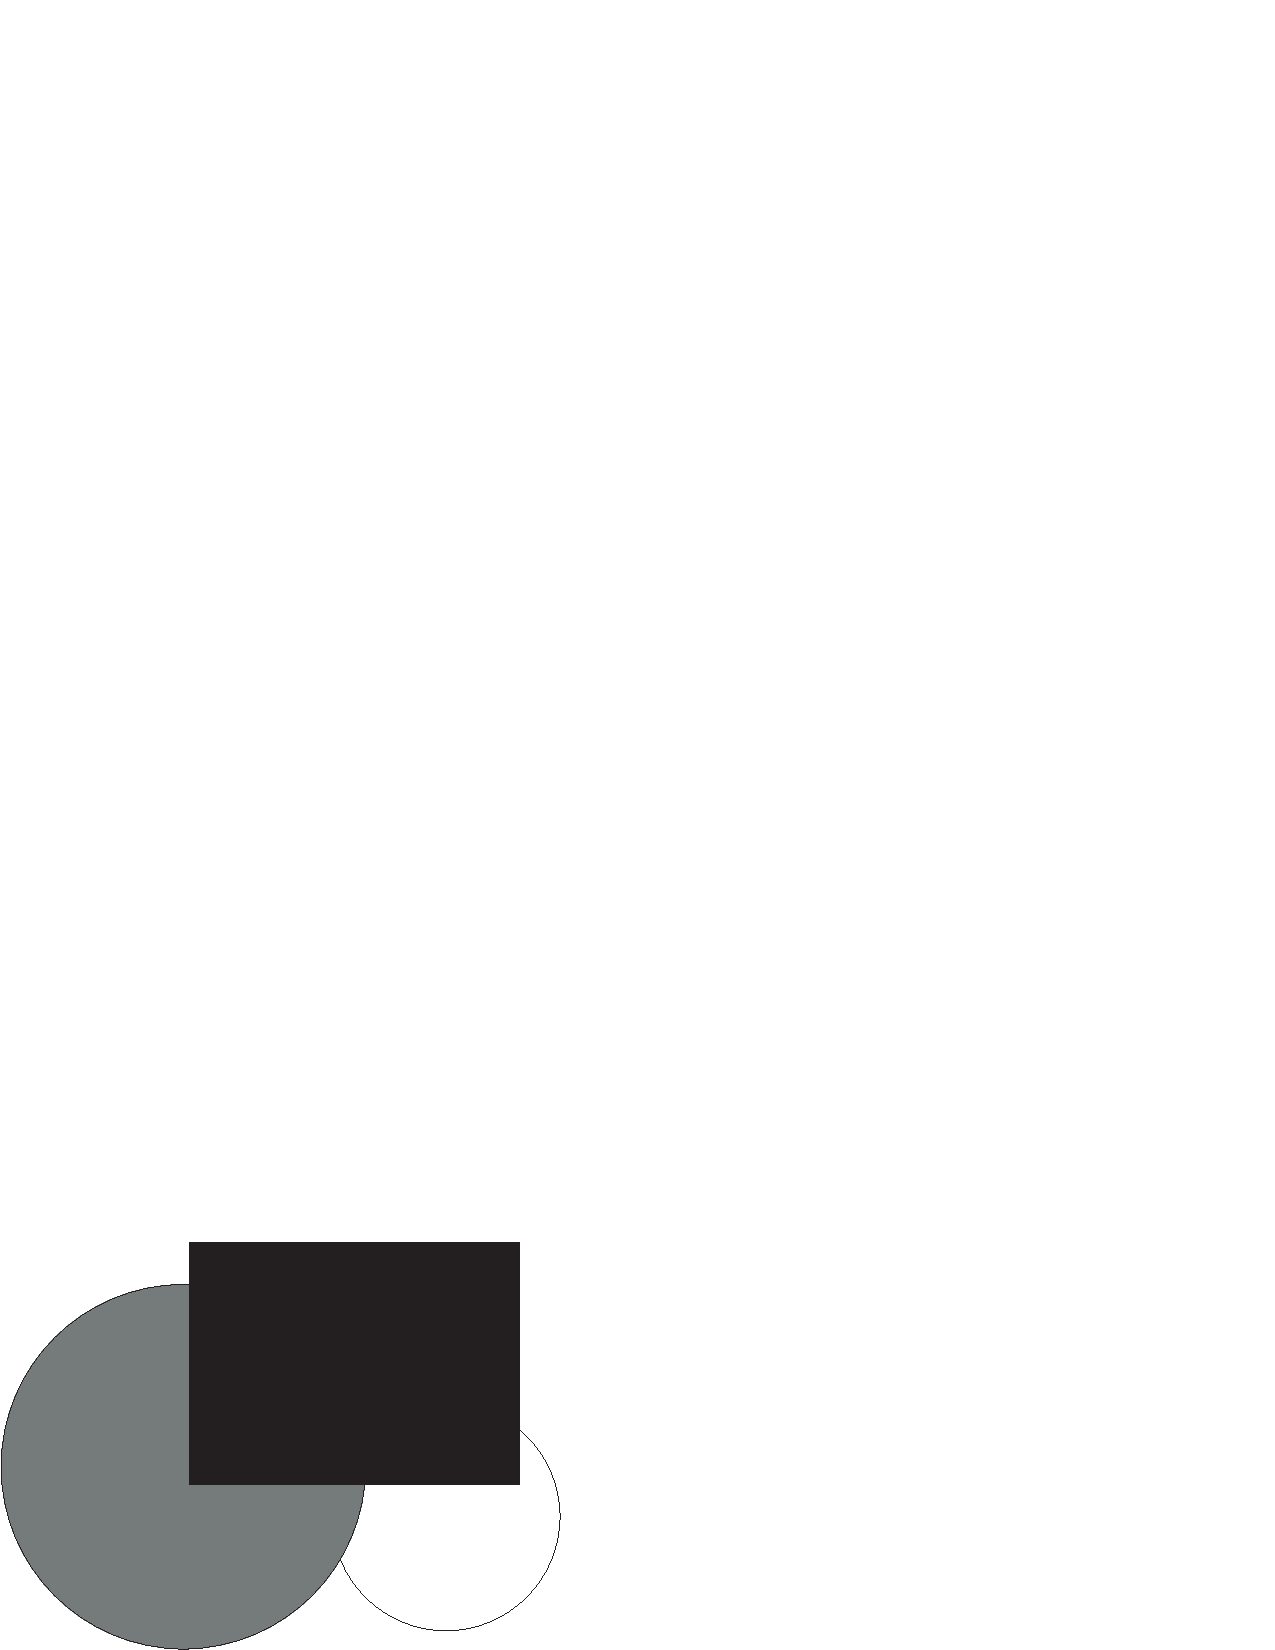
\includegraphics[width=.5\textwidth]{example_fig}
  \caption[An example figure.]{An example figure. If the caption is
    shorter than one line, it is centered. If it goes over more than
    one line, it is left and right justified. Furthermore, it is
    suggested that an alternative short caption is given in order to
    produce a good list of figures.}
  \label{fig:example}
\end{figure}

\begin{table}[tbp]
  \centering
  \begin{tabular}{c|c}
    Age  & IQ  \\ 
    \hline
    10   & 100 \\
    20   & 100 \\
    30   & 150 \\
    40   & 100 \\
    50   & 100
  \end{tabular}
  \caption{An example table.}
  \label{tab:example}
\end{table}

The captions are placed \emph{below} both for the figures and the
tables. The caption is set in 9pt. If the caption is shorter than one
line, it is centered.

\section{Quotes}
\label{sec:Quotes} % this allows you to refer to this section number using \ref{sec:Quotes}

Quotes are inserted using the standard \LaTeX\ \texttt{quote}
environment. The environment has been changed so that a 9pt font is
used:

\begin{quote}
  ``And I looked, and, behold, a whirlwind came out of the north, a
  great cloud, and a fire infolding itself, and a brightness was about
  it, and out of the midst thereof as the colour of amber, out of the
  midst of the fire. Also out of the midst thereof came the likeness
  of four living creatures.''
\end{quote}

\section{Lists}
\label{sec:lists}

Point lists and enumerated lists are made by using the standard
\texttt{itemize} and \texttt{enumerate} environments, respectively.
The spacing is going to be changed in accordance with the specification. For
\texttt{itemize}, the results look like this:
\begin{itemize}
	\item First item.
	\item Second item. Here I will put some long text, just to illustrate.
	  Here I will put some long text, just to illustrate. Here I will put
	  some long text, just to illustrate. Here I will put some long text,
	  just to illustrate.
	\item Third item also has subitems:
	  \begin{itemize}
		  \item First subitem.
		  \item Second subitem.
		  \item Third subitem.
	  \end{itemize}
\end{itemize}
and for \texttt{enumerate} like this:
\begin{enumerate}
	\item First item.
	\item Second item. Here I will put some long text, just to illustrate.
	  Here I will put some long text, just to illustrate. Here I will put
	  some long text, just to illustrate. Here I will put some long text,
	  just to illustrate.
	\item Third item also has subitems:
	  \begin{enumerate}
		  \item First subitem.
		  \item Second subitem.
		  \item Third subitem.
	  \end{enumerate}
\end{enumerate}

You may also want to use descriptive lists
\begin{description}
	\item[First] the first item.
	\item[Second] the second item. Here I will put some long text, just to illustrate.
	  Here I will put some long text, just to illustrate. Here I will put
	  some long text, just to illustrate. Here I will put some long text,
	  just to illustrate.
	\item [What now] the third item also has subitems:
	  \begin{enumerate}
		  \item First subitem.
		  \item Second subitem.
		  \item Third subitem.
	  \end{enumerate}
\end{description}


\section{Bibliographic References}

You should cite articles~\cite{Askvall1985}, books~\cite{Card1983},
anthologies~\cite{Lancaster1985} and web publications~\cite{Meldon1997}
like this. There is always an issue referencing web pages. Currently
we suggest that you use the HiG Website~\cite{HiG:Website}.


A particular bibliography style file for GUC named
\texttt{gucthesis.bst} has been developed based upon the
standard Bib\TeX\ \texttt{unsrt} style.


\bibliographystyle{gucthesis}
\bibliography{BachelorExample}



\appendix %after this line all chapters will have leters instead of numbers

\chapter{Meetings}

You can include an Appendix of the log of your meeting for example

\GUC, 
\comment{so what}

\todo{task \#1}
This is a todo-task we need to get done.

\end{document}